\documentclass[11pt,twoside]{article}
\usepackage{geometry}
\usepackage{enumerate}
\usepackage{latexsym,booktabs}
\usepackage{amsmath,amssymb}
\usepackage{graphicx}
\usepackage[singlespacing]{setspace}
\usepackage{multirow}
\usepackage{multicol}
\usepackage{longtable}
\usepackage{tabularx}
\usepackage{makecell}
\usepackage{float}
\usepackage{hyperref}
\usepackage[skip=0.5\baselineskip]{caption}

\geometry{a4paper,left=2cm,right=2.0cm, top=2cm, bottom=2.0cm}

\newtheorem{Definition}{Definition}
\newtheorem{Theorem}{Theorem}
\newtheorem{Lemma}{Lemma}
\newtheorem{Corollary}{Corollary}
\newtheorem{Proposition}{Proposition}
\newtheorem{Algorithm}{Algorithm}
\numberwithin{Theorem}{section}
\numberwithin{Definition}{section}
\numberwithin{Lemma}{section}
\numberwithin{Algorithm}{section}
\numberwithin{equation}{section}
 
\newenvironment{modelsets}
  {\paragraph{Sets}\mbox{}\par\nobreak\vspace{-0.5\baselineskip}
   \begin{tabular}{@{}l @{\quad} p{0.85\linewidth}@{}}}
  {\end{tabular}\par\vspace{\baselineskip}}
 
\newenvironment{modelparams}
  {\paragraph{Parameters}\mbox{}\par\nobreak\vspace{-0.5\baselineskip}
   \begin{tabular}{@{}l @{\quad} p{0.85\linewidth}@{}}}
  {\end{tabular}\par\vspace{\baselineskip}}


\begin{document}

\pagestyle{empty}

% =============================================================================
% Title page
% =============================================================================
\begin{titlepage}
\vspace*{.5em}
\center
\textbf{\large{The School of Mathematics}} \\
\vspace*{1em}
\begin{figure}[!h]
\centering

\includegraphics[width=180pt]{CentredLogoCMYK.jpg}
\end{figure}
\vspace{2em}
\textbf{\Huge{Pairing Caregivers as a Preliminary Step in the Home Healthcare Routing and Scheduling Problem}}\\[2em]
\textbf{\LARGE{by}}\\
\vspace{2em}
\textbf{\LARGE{Nolan Willoughby}}\\
\vspace{6.5em}
\Large{Dissertation Presented for the Degree of\\
MSc in Operational Research}\\
\vspace{6.5em}
\Large{August 2026}\\
\vspace{3em}
\Large{Supervised by\\Dr. Jörg Kalcsics}
\vfill
\end{titlepage}

\cleardoublepage

% =============================================================================
% Abstract, acknowledgments, and own work declaration
% =============================================================================
\pagestyle{plain}
\setcounter{page}{1}
\pagenumbering{roman}

\begin{center}
\Large{Abstract}
\end{center}
Home Healthcare is the process by which certain health-related services are provided to patients in their home, and is a service that is becoming increasingly essential due to several demographic and cultural shifts. Due to the ever more critical nature of the work and the logistical complexity of performing that work, this domain presents great potential for the use of Operations Research techniques. The Home Healthcare Routing and Scheduling Problem is a problem in Operations Research combining aspects of several canonical problems in the Operations Research literature with the aim of optimizing the assignment of caregivers to visits (scheduling) and the sequencing of each caregivers' visits (routing). This work focuses on introducing a preliminary step to an existing Routing and Scheduling heuristic that pairs a subset of available caregivers to simplify downstream planning of visits requiring the presence of multiple caregivers in the context of a particular home healthcare provider. A multi-objective Mixed-Integer Linear Program is formulated with considerations for the geospatial distribution of caregiver assignments relative to that of demand and the shift pattern of caregivers. This model is then implemented and feasible caregiver assignments are derived, tested, and evaluated with the provider's existing routing and scheduling heuristic. 

\clearpage

\begin{center}
\Large{Acknowledgments}
\end{center}

I would like to thank my family, including those no longer with us since my arrival in Edinburgh, for all of their love and support, both as it related to this dissertation and in general. I would not be who or where I am today without you guys, and, while I do not necessarily understand what I did to deserve you, I appreciate you all dearly. I would also like to thank my supervisor, Jörg, for his direction, insight, and wit. Your supervision was essential to ensuring this project was successful, and I thank you for that. Similarly, I would like to thank every member of the staff under whom I have had the opportunity to learn and grow over this last year. The staff here was the primary reason I applied to and chose to enroll in this program, and I am grateful at having had the opportunity to learn from you guys. I hope that the university and its leadership come to realize this sooner rather than later and compensate you all appropriately according to the value you provide to the university. Finally, I would like to specifically express my love and gratitude to Jasper, Oliver, and the late Goldie, who are the best dogs ever and never fail(ed) to brighten my day. 

\clearpage

\begin{center}
\Large{Own Work Declaration}
\end{center}

I attest that I am the sole author of this thesis and that all the content within it is my original work, except for any instances where I have clearly indicated otherwise in the text. 

\cleardoublepage



% =============================================================================
% Table of contents, tables, and pictures (if applicable)
% =============================================================================

\tableofcontents
\clearpage
\listoftables
\listoffigures
\cleardoublepage

\pagenumbering{arabic}
\setcounter{page}{1}

\nocite{*}
\bibliographystyle{abbrv}
\clearpage

\section{Introduction}
\label{sec.intro}
Home Healthcare is the process by which certain health-related services, typically including nursing care, prescription and other medical supply delivery, and/or assistance with day-to-day activity, are provided to patients in their home \cite{al-hamad}. Among the requirements of each visit is the number of caregivers required to be present, which is typically either one or two \cite{Mankowska2014}. Home Healthcare operations involve a complex logistics network which require involved planning and present a high-potential opportunity for Operations Research techniques. Operations Research is the branch of applied mathematics dealing with the formulation and solving of decision problems. Among the Operations Research literature is a vast amount of research dedicated to the Home Healthcare Routing and Scheduling Problem, which extends the Vehicle Routing Problem, another extensively researched problem structure in the domain of Operations Research, to the specific requirements of Home Healthcare operations. The Home Healthcare Routing and Scheduling Problem produces caregiver schedules, i.e. lists of visits for caregivers in the Home Healthcare provider to serve, and routes for caregivers to take between their scheduled visits. 

This work involves the development of a preliminary step to this Home Healthcare Routing and Scheduling Problem as applied in practice by a certain Home Healthcare provider. Using multi-objective Mixed-Integer Linear Programming techniques, candidate caregiver units are assigned on a day to day basis, with units ranging in size from one to three depending on the type of visit the unit is meant to serve with regard to number of caregivers required and the shift pattern of the caregivers in the unit. Assignments are optimized to maximize the potential number of visit minutes which will be served that day by a caregiver or caregivers already familiar to the client and to minimize the potential travel required of caregivers to join the other members of their unit and travel to their day's visits. The design of the model addresses caregiver shift patterns, geospatial distribution of caregivers and clients, the share of visits which require one caregiver and that which require two, and further client preferences. The model is implemented on a two-week data sample from the relevant Home Healthcare provider, with assignments further evaluated for their effect on a Routing and Scheduling heuristic developed for said provider.

The rest of the report is organized accordingly. Section \ref{sec:background} will provide a review of relevant literature to the project in the interest of contextualizing the general nature of the work being done. Section \ref{sec:prob} will formally define the problem being addressed by this work in the specific context of one Home Healthcare provider. Section \ref{sec:meth} will cover the various items necessary to consider when addressing this problem, the specific approach chosen, and the way in which that approach was implemented, while Section \ref{sec:res} will provide detailed computational results of the methodology as implemented. Section \ref{sec:conc} will conclude by briefly reviewing the accomplishments detailed throughout, detailing limitations of the work, and noting recommendations for its future development.
\clearpage

\section{Background}
\label{sec:background}
To better inform the work conducted, it is necessary to first understand the literature context in which it is placed. This chapter will provide such context by reviewing relevant literature on Home Healthcare as a service and industry, Operations Research and its relevant canon problem structures, and applications of Operations Research to this and other healthcare contexts. 
\subsection{Home Healthcare}
Home Healthcare is the process by which certain health-related services are provided to patients in their home. These services typically involve nursing care, though can also consist of prescription and other medical supply delivery as well as assistance with day-to-day activity \cite{al-hamad}. These services provided by Home Healthcare models are becoming increasingly essential as demographic changes yield older populations, greater geographical dispersion relative to both family and central hospital campuses, and a general preference toward aging in place. Additionally, Home Healthcare services can prove essential to modern healthcare systems by enabling personalized, expert care for patients with chronic illness, mobility challenges, and post-operation recovery needs who may not otherwise be able to receive such quality care \cite{atta25, Mankowska2014}.

Consequently, the importance of Home Healthcare providers, i.e. groups providing these services, is of increasing social interest. These groups face several operational challenges to meet the needs of their client base, and must do so with efficiency to ensure competitive advantage in a market system. Among the challenges of these groups is the need to find ways to efficiently provide diverse services requiring differing numbers and types of caregivers \cite{begur97, Mankowska2014}. Not only must these services be provided by varying numbers of caregivers with various qualifications, they must also be delivered within strict time windows according to patient care needs \cite{begur97}. Given the operational complexity and social importance of these operations, the operations of Home Healthcare providers are a domain with high-potential for Operations Research applications.

\subsection{Operations Research and its Relevance}

Operations Research is the branch of applied mathematics dealing with the formulation and solving of decision problems. As such, it presents an area of particularly enticing growth potential for operations involving multiple, complex decisions. As discussed in the immediately preceding section, the field of Home Healthcare is one such domain, as it involves decisions on the assignment of caregivers in the system to visits and the routing of caregivers between visits, and must consider the qualifications of caregivers, the requirements of each visit, and the time windows in which each visit must be completed. As such, there is a great deal of potential for the field of Operations Research when applied to the domain of Home Healthcare, as can further be understood through the lens of textbook examples of Operations Research applications from the literature. 

\subsubsection{The Vehicle Routing Problem}
The first relevant problem structure from the Operations Research canon to note is the Vehicle Routing Problem. Formally, the Vehicle Routing Problem is defined by a set of customers, each with known demand, a set of vehicles available to serve those customers, and known costs for serving each customer both individually and following from a prior customer. The objective of the Vehicle Routing Problem then is to assign each vehicle a subset of the customers and an order, i.e. routing, by which each vehicle is to serve its assigned customers such that the overall cost across all vehicles' assigned routes is minimized. This problem typically involves capacitated vehicles, i.e. each vehicle is limited in the amount of demand it is able to service, while otherwise resembling an extended version of the Traveling Salesman Problem \cite{NELSON1985}. While the Vehicle Routing Problem is critical to efficient operations in several industries, solving the Vehicle Routing Problem is NP-hard. This has resulted in a great deal of research dedicated to solution methodologies for the Vehicle Routing Problem that take advantage of computing advances and the practical, application contexts in which they arise \cite{TanetYeh}. 

Exact solution methods based on either Mixed Integer Linear Programming, Dynamic Programming, or Constraint Programming have seen increased prevalence corresponding with increased computing power, and these techniques are typically further supplemented by techniques such as column generation to improve their performance. These methods are practically limited by the scale of the application; because the Vehicle Routing Problem is NP-hard, exact methods are practically limited to small scales. By contrast, heuristic and meta-heuristic solution methods are not limited in scale and as such continue to dominate the literature. These techniques, notably including Simulated Annealing, variations of Neighborhood Search, Tabu Search, Genetic Algorithms, and Ant Colony Optimization, are designed to produce near-optimal solutions within a given runtime \cite{TanetYeh}. 

Two notable variants of the Vehicle Routing Problem introduce time windows (canonically known as the Vehicle Routing Problem with Time Windows) and heterogenous vehicle fleet compositions (canonically known as the Vehicle Routing Problem with Heterogenous Fleets) as additional considerations in the routing process. This first structure extends the existing Vehicle Routing Problem to enforce time windows within which a visit must be scheduled \cite{desroisiers-solomon}. This extension allows the same Vehicle Routing framework to extend to applications where the services demanded by each customer node are time-sensitive, i.e. the node must be visited by a vehicle and service completed by that vehicle within a given time window. Due to industry trends, this variant of the Vehicle Routing Problem is a particular focus of recent literature \cite{TanetYeh}. Meanwhile, the latter structure extends the Vehicle Routing Problem to consider cases where the fleet of vehicles available to travel to and service customers contains subsets of vehicles with unique characteristics that constrain either their ability to travel, their ability to provide certain services, or both \cite{WassanOsman}. These extensions serve to further constrain an already difficult problem, but are essential to ensuring its practical applicability. This is borne out in the case of Home Healthcare, where visits must be serviced in specific time windows and caregivers have unique attributes and/or qualifications that dictate which visits and which routings they are able or unable to perform.

A final extension of the Vehicle Routing Problem to consider is the introduction of synchronizations. For the purposes of this context, synchronizations will refer specifically to operation synchronizations, which formally dictate that the delivery of a service to a given customer by a given vehicle must coincide within a given time window with the delivery of another service to a given customer by another given vehicle, with the note that the customers in this case may be the same customer or two separate customers. In other words, operation synchronizations involve coordinating routes and schedules such that multiple vehicles arrive at a designated location within a specific time relative to each other. Naturally, this consideration requires careful, deliberate modelling techniques, as the selection of each effected vehicles' individual routes must now be made in relation with all other effected vehicles' routes, affecting the feasibility of routing both upstream and downstream of the required operation synchronization(s). Accordingly, while exact and heuristic approaches varying significantly depending on context, one through line in the literature is the difficulty in solving Vehicle Routing Problems with Synchronizations at scale, both in modelling and computational terms \cite{drexl}. 

\subsubsection{Matching and Assignment Problems}
Another relevant problem structure to consider from the Operations Research canon are Matching Problems. In the most general sense, Matching Problems are defined by a general, undirected graph $G = (V, E)$, where $V =$ the set of nodes and $E \subseteq V \times V$ is the set of edges between nodes. A matching $M \subseteq E$ is then a subset of edges such that each node in the graph is incident to at most one edge in $M$. Matching Problems are then problems in which a "best" matching must be derived, with the details of what constitutes a so-called "best" matching left to the context of the problem. Matching Problems that associate a cost or benefit $c_e$ with including an edge $e$ in the matching $M$ are known as Assignment Problems, and typically involve finding a matching $M$ such that the cost or benefit of said matching $\sum\nolimits_{e \in M} c_e$ is minimized or maximized respectively. These problem definitions notably involve one-to-one matching and assignment; they can be generalized to involve one-to-many in the Generalized Assignment Problem \cite{burkard}.

Matching and Assignment Problems can be solved using Mixed-Integer Linear Programming, with binary decision variables associated with each edge $e \in G$; constraints ensuring, among other restrictions specific to the problem context, that each node $v \in G$ is incident to at most one of the edges chosen; and an objective of optimizing for some definition of a "best" matching, which, in the case of Assignment Problems, naturally remains to maximize the benefit or minimize the cost of a chosen matching. Mixed-Integer Linear Programming approaches extend well to the Generalized Assignment Problem, as the formulation can typically be easily adapted by relaxing the right hand side of constraints relating to the maximum number of edges a node may be adjacent to in the final matching \cite{burkard}.

While Mixed-Integer Linear Programming approaches work for any problem instance in this class, they are not necessarily the most efficient approach to take. Combinatorial Optimization techniques for this family of problem seek instead to exploit the characteristics of the graph $G$ to find optimal solutions more efficiently. In the case of the Maximum Cardinality Matching Problem, which seeks to find the matching $M$ such that $M$ contains the greatest possible number of edges $e \in G$, this typically involves iteratively deriving $M$-augmenting paths from an arbitrary initial matching \cite{burkard}. This technique is particularly adept in cases where $G$ is a bipartite graph (and indeed works in $\mathcal{O}(nm)$, where n is the number of nodes and m the number of edges in the graph), though can be adapted to a general graph \cite{Edmonds_1965}. The Hungarian Algorithm extends this approach to Assignment Problems in $\mathcal{O}(n^3)$ by iteratively reducing the graph according to edges' node potentials and finding a corresponding maximum cardinality matching, though this algorithm only works if the graph is bipartite \cite{hungary, munkres}.

\subsection{Application of OR to Healthcare Contexts}

While Operations Research was initially developed in the context of supporting the Allied effort in World War II, its applicability to other domains where operations are complicated and success dependant on beneficial decision-making has been recognized. One such field is that of healthcare. There exists a great deal of literature on Operations Research as applied to the domain of healthcare, with the majority dedicated to the use of simulation techniques meant to analyze the efficiency of healthcare processes and test the effect of potential changes on the overall system and its efficiency. That said, the presence of optimization modelling in the industry is not entirely lacking, as there exist several examples in the literature of such modelling being used to improve the efficiency with which limited healthcare-related resources are deployed \cite{mustafee13}.

One example of optimization-driven decision support in healthcare is that of Operating Room Scheduling, which concerns assigning surgical cases to a hospital's limited operating room capacity so as to balance competing objectives such as minimizing patient waiting time, maximizing throughput, and controlling overtime costs. Given both the scale of investment tied up in operating room capacity and the direct link between surgical throughput and hospital revenue, this problem is well-represented in the Operations Research literature. This body of work spans both the strategic and tactical planning of surgical block schedules and the more operational, day-to-day sequencing of individual cases, and draws on much of the modelling techniques discussed in the prior section, including Mixed-Integer Linear Programming formulations and a range of heuristic and meta-heuristic solution approaches. This follows from the fact that this problem can be abstracted to a General Assignment Problem. Unique to this application domain, however, is the consideration of healthcare-specific factors such as the effect of Operating Room operations on other units within a hospital, the uncertainty associated with non-elective or ad-hoc procedures, and the practical impracticalities of purely efficient solutions due to their potential for deadly consequences under the observation of certain uncertainties \cite{CARDOEN2010}.

A second example comes from the field of dispatching Emergency Medical Services. Where operating room scheduling is typically addressed as a static or cyclical planning problem, the dispatch of ambulances to incoming calls and the ongoing relocation of idle vehicles across a coverage area are inherently dynamic and stochastic decision problems, made under considerable uncertainty as to the timing and location of future demand. While there still exists scope for traditional, Mixed-Integer Linear Programming-based optimization approaches to strategic ambulance location, the dynamic nature of the domain area has led to the innovative use of techniques such as approximate dynamic programming, Markov Decision Processes, and simulation-based optimization methods to handle dynamic ambulance management, or the dispatch and relocation of ambulances subject to real-time updates in emergencies and ambulances' operational states. Again, a commonality of these applications are the need to consider factors beyond overall efficiency or cost, as decisions taken fundamentally affect the livelihoods of people involved \cite{Jagtenberg2017}. 

\subsubsection{The Home Healthcare Routing and Scheduling Problem}

The applicability of Operations Research to healthcare settings has not been limited to these applications. Indeed, the aforementioned applicability of Operations Research to Home Healthcare settings has been well-documented in the literature as a unique class of problem known as the Home Healthcare Routing and Scheduling Problem. This problem was first identified in 1997 by Begur et al, who developed a heuristic Spatial Decision Support System tailored to advise an operation covering a large area in Alabama on optimized daily routes and schedules \cite{Masmoudi2024, begur97}. In the intervening years, the literature has developed substantially, with at least 80 publications developing the understanding of the problem and its potential solution methodologies published between 2019 and 2023 \cite{Masmoudi2024}. 

The Home Healthcare Routing and Scheduling Problem may be seen as yet another extension of the Vehicle Routing Problem, including time windows, synchronization, heterogenous fleets (i.e. caregiver skill requirements), multiple depots (i.e. routes may start and end in multiple locations rather than one centralized depot as in the original definition of the Vehicle Routing Problem), and other constraints related specifically to healthcare applications such as continuity of care \cite{atta25}. This problem further differs from the traditional Vehicle Routing Problem as certain clients must be visited multiple times, while the Vehicle Routing Problem traditionally visits customers strictly once \cite{Mankowska2014}. 

Objectives of the Home Healthcare Routing and Scheduling Problem typically include minimizing travel and related costs; maximizing some measure of patient satisfaction; maximizing some measure of caregiver satisfaction, including by optimization for workload balancing; and minimization of unscheduled visits. As mentioned previously, formulations are frequently constrained by visits' requirements of caregivers (both in number and in skills), time windows in which visits must be made, continuity of care, caregiver lunch breaks and workload, and visit precedence requirements, among others. Solution techniques share a great deal with those mentioned in relation to the Vehicle Routing Problem, though some differences emerge. Notable is the frequency with which exact methods are combined with heuristics to handle large instances while dealing with particular practical constraints. Another notable difference is the frequency with which the problem is decomposed in a multi-stage solution approach. This again allows solutions to be generated with greater efficiency by considering certain constraints at different stages of the solution process \cite{atta25}. 

For a time, the preeminent approach to the Home Healthcare Routing and Scheduling Problem was that put forward in 2014 by Mankowska et al \cite{ceschia25}. Their formulation sought to address several disparities in formulations across the contemporary literature, namely whether homogenous or heterogenous teams of staff members were considered, whether synchronization of interdependent services were considered, the particular objectives pursued in optimizing the problem, and the methodology used for obtaining its solution. This was done by formulating to consider heterogenous staff, time-dependence of services, whether single or double services are required (i.e. whether a visit requires one or two caregivers present), and a balance of cost and service objectives (namely total distance traveled, overall tardiness of services delivered, and maximum tardiness of services delivered, which were parametrized in a single objective function with deliberate choices of $\lambda$ enabling the objective to represent specific objectives including economic tradeoff of cost and service quality), while enforcing caregiver qualification requirements and the fulfillment of all demanded services \cite{Mankowska2014}. As their Mixed-Integer Linear Programming formulation could be shown to contain the NP-hard multiple Traveling Salesman Problem with Time Windows, they put forward an Adaptive Variable Neighborhood Search heuristic as a suitable solution technique. As a final note on Mankowska et al.'s 2014 work, they put forth several benchmark Home Healthcare Routing and Scheduling data instances based on their formulation, allowing for their and future formulations to be tested against a unified, representative dataset \cite{Mankowska2014}. 

This formulation served as a benchmark singular, unified formulation of the Home Healthcare Routing and Scheduling Problem for an extended period in the literature. In 2025, Ceschia et al. aimed to further supplement the Mankowska formulation by again unifying the further practical constraints observed in the literature left unaddressed by the existing benchmark formulation into a single, unified formulation \cite{ceschia25}. This new formulation built on Mankowska's existing benchmark by considering patient preference of caregivers, both in incompatibilities and preference; the ability for caregivers' routes to start from multiple locations rather than one, centralized depot; further consideration of caregiver workload (including relative to other caregivers), shift patterns, lunch breaks, overtime, and waiting time; and the addition of multiple candidate time windows per patient. Additionally, the new formulation expanded the objectives considered from the original three to 10, with these specifically being framed as costs to minimize across a similarly parametrized objective function \cite{ceschia25}. These objectives were as follows:
\begin{enumerate}
	\item Total distance traveled
	\item Overall tardiness of services delivered
	\item Maximum tardiness of services delivered
	\item Total overtime required of caregivers
	\item Total waiting time required of caregivers at patients' locations
	\item Maximum idle time of caregivers
	\item Total absolute deviation of caregiver working time from average
	\item Total penalty cost of visits served by caregivers different from a client's preferred caregivers
	\item Total penalty cost of caregivers skipping lunch breaks
	\item Total penalty cost of skipping "optional" patients
\end{enumerate}

Beyond this, Ceschia et al. put forth both a Mixed-Integer Linear Programming exact approach and a Simulated Annealing heuristic as potential solution methods for their unified formulation. They tested this against Home Healthcare Routing and Scheduling data instances generated by their own generator updated according to their new unified formulation and supplementary to those of Mankowska et al. \cite{ceschia25}. 

\clearpage

\section{Problem Statement}
\label{sec:prob}
As a first step in an engineering design process, it is important to formally define the nature and objective of this work. This case involves the scheduling and routing decisions faced by a certain Home Healthcare Provider. The provider employs approximately 50 caregivers and services approximately 150 clients. Caregivers may work either a full-time, morning, or afternoon shift pattern, and each caregiver is available for a given subset of days in the planning window. This information is known and decided on a two week planning horizon due to minimum work thresholds set by the UK Home Office for caregivers on sponsored work visas. Caregivers may or may not have the ability to drive, with driving caregivers able to cover a larger service area than non-drivers. That said, caregivers are generally not compensated for time spent on their shift traveling, though there can be exceptions to this rule for certain, extenuating circumstances. Additionally, approximately 90\% of all caregivers identify as female, and all caregivers share functionally equivalent qualifications sufficient to perform any visit the provider may have commitment to perform. 

Clients typically require between three and five visits daily, with most visits lasting between 30 and 60 minutes. Each of these visits must occur within a given time window, and each visit requires either one or two caregivers present. Clients typically prefer visits to be performed by caregivers already known to the client, and clients can specify a preference on the gender of the caregiver(s) assigned to perform their visit(s). Clients and their caregivers are spread across the provider's service area, which broadly covers three municipalities. The distribution of clients and caregivers across this area is not uniform, and this disparity must be taken into account when routing and scheduling visits. On any given day, the total duration of all visit minutes requiring two caregivers present represents about 40\% of the total duration of all visit minutes which must be served on that day. 

The problem in this case, therefore, is to identify an optimal or near-optimal allocation or scheduling of caregivers to the set of visits the provider is committed to service and the order or routing in which the caregivers ought to perform their assigned visits. Attention must be paid to the shift pattern that assigned caregivers work, whether assigned caregivers are able to drive or are paired with another caregiver able to drive, and whether caregivers match the gender preferences of the client. Because all caregivers functionally share the same qualifications, there is no need in this case to consider visits that can only be performed by a subset of caregivers, with the exception of cases with an expressed gender preference. This is in contrast to most formulations of the Home Healthcare Routing and Scheduling Problem, which constrain a caregiver's scheduling according to whether that caregiver has the requisite qualification(s) to perform the tasks of each visit. With the problem formally defined, it is then possible to lay forth a modelling approach meant to solve the problem as defined.

\clearpage

\section{Methodology}
\label{sec:meth}
Having now defined the problem, this chapter will detail the methodology considered and ultimately chosen to address the problem. Discussion will start with a review of the various approaches considered as potentially applicable to the problem, followed by an overview of the approach deemed most appropriate to the context. The rest of the chapter will then focus on the specifics of the ultimate design approach taken.

\subsection{Design Considerations}

The first consideration to make in designing a model for this problem is to consider the objectives of involved parties. In this case, the Home Healthcare provider has the objective of providing its clients their required services to a satisfying degree, while remaining profitable and potentially growing its business. The provider's caregivers, meanwhile, desire solutions which provide routing and scheduling that does not overextend their faculties, is generally fair caregiver to caregiver, and increases their share of working hours which are paid. Finally, the provider's clients want quality, timely visits from caregivers they know and trust. Potential objectives of this Home Healthcare Routing and Scheduling model therefore include maximizing the number of visits served (thereby minimizing the number of unallocated visits), minimizing the cost incurred of routings and schedulings, minimizing the number of visits and/or amount of travel individual caregivers must perform, minimizing the difference in workload and/or travel between the caregivers with the highest and lowest observed workload and/or travel, minimizing the amount of uncompensated time (driving and idle time) experienced by caregivers, maximizing the number of visits serviced by a caregiver or caregivers which are known by the corresponding client, and minimizing the time window violations or tardiness of a routing and scheduling. The least computationally complex model would choose exactly one of these objectives over which to optimize, while considering multiple of these listed objectives would potentially result in better solutions on a system level at the cost of added computational complexity.

In terms of conditions solutions must meet and that a model must therefore consider as constraints, the first of these is to consider the fact that certain visits require the presence of multiple caregivers. If each caregiver is routed and scheduled individually, the model must consider how individual caregivers' routes and schedules can synchronize at each visit requiring the presence of multiple caregivers. This would require the model to incorporate several aspects of the computationally difficult Vehicle Routing Problem with Synchronizations. The synchronization approach would add significant operational and computational complexity, as well as a lack of schedule and routing robustness in the event of unanticipated disruptions. In return, solutions would approach a higher degree of optimal efficiency. This approach is therefore particularly suited to applications in which the share of visits requiring multiple caregivers is low, as this would require fewer synchronizations and suffer fewer consequences in the event that synchronizations are disrupted by unforeseen factors. Another option would be to pair caregivers for the day as a preliminary step to routing and scheduling. This would likely lead to less efficient solutions than the synchronization approach may yield. As a trade-off, solutions would be less complex both operationally and computationally, while also being more resilient to unanticipated disruptions. This approach is therefore better suited to contexts in which the share of visits requiring multiple caregivers is high, as not only do those contexts present more opportunity to incur negative outcomes in the event of synchronizations being disrupted, they also would likely yield synchronization-based solutions with sufficient synchronization occurrences as to be similarly efficient to solutions where daily caregiver pairs are determined as a preliminary to routing and scheduling. 

Another important consideration must be made regarding the shift patterns of caregivers. In a synchronization-based approach, this consideration is trivial, as each caregiver is routed and scheduled independently and can therefore be assigned to visits with or without other caregivers freely within their available hours and constrained out of use without those hours. However, if an approach pairing caregivers for the day is implemented, shift patterns must be explicitly considered to avoid pairing caregivers with incompatible shift patterns and maximize the utility of each pairing (i.e. ensure members of a caregiver pairing are active for the majority of the others' shifts). In the day-long pairing approach to considering visits with multiple caregivers, shift patterns might be accounted for by total enumeration of potential pairings, including pairings of three caregivers in which two caregivers of alternate shift patterns are paired with a full-time caregiver, and optimizing the selection of these pairings; further granulating the daily assignment by creating separate daily assignments for the morning and afternoon; or as a hybrid synchronization approach in the downstream routing and scheduling model where caregivers whose partners are inactive can synchronize on an as-needed basis and otherwise perform single caregiver visits.

A further consideration for the daily pairing assignment approach is the geospatial distribution of assignments. The simplest approach both with regard to ease of formulation and computational complexity would be to not consider this distribution at all and make location-blind assignments. Since caregiver assignments are made as a preliminary to routing and scheduling, making assignments without accounting for the locations of caregivers and clients may result in inefficient routings due to caregiver and/or pairing locations being located far from the clients those caregivers and/or pairings are meant to serve. One approach to consider geospatial distributions would be to group clients into neighborhoods or localities and ensure that each locality is assigned sufficient caregiving units to perform the visits in that locality. This would require the model to make additional decisions beyond just which caregivers to pair and which to assign as individuals; the model would also have to assign each of these units to a locality while considering the travel required for a unit to move from its origin(s) to its assigned locality. Consequently, this would increase computational complexity. If the visits requiring a single caregiver are spread with a roughly similar geographic distribution as those requiring two caregivers, it may be appropriate to simply consider that the number of units assigned to each locality is sufficient regardless of unit size, while disproportionate distributions of these two visit types would require explicit, separate consideration of the spread of pair unit locality assignments and solo unit locality assignments. 

An additional consideration is the question of accounting for clients' gender preference. In a synchronization approach, this consideration must naturally be made as a constraint on which caregivers may be assigned to each visit in the scheduling part of the problem. In the daily pairing assignment approach, this consideration may be made by ensuring a sufficient share of pair and solo assignments are made to meet the gender requirements of a day's visits. Conversely, in the event that gender preferences are largely in line with the population of caregivers, assignments can be made without considering caregiver gender, leaving gender preference to be considered solely as a scheduling constraint.

Lastly, an overarching consideration must be made for the complexity and scope of the model in the context of how and by whom it will be used. This is to say, the computational and technical complexity of the model should be tailored to the ease, frequency, and speed with which the model must provide its solutions, and the model must be usable and comprehensible to the person or people who use it. This consideration influences how each of the previous considerations are made and what design decisions are derived for each. In short, the design of the model must result in a tool that is practical for the use case for which it is designed
\subsection{Modelling Approach}
Given these design considerations, the following modelling approach is put forward. The scope of this work will be to assign caregivers to paired or solo caregiving units on a daily basis. This follows from the provider's relatively large share of visits requiring two caregivers, allowing for day-long caregiver assignments of this manner to be sufficiently efficient. This will be accomplished by the formulation of a Mixed-Integer Linear Program similar to a standard General Assignment Problem formulation. This Mixed-Integer Linear Program will serve as a preliminary to a downstream routing and scheduling heuristic out of the scope of this work. As there are several potential objectives and the current downstream heuristic can be run in relatively short runtimes, a constraint-based multi-objective approach will be implemented.

Following this overall approach to the problem in scope, several considerations must explicitly be made. Because of the relatively low share of caregivers on part-time shift patterns, feasible units will be totally enumerated as a pre-processing step, and the model will then optimize the assignment of each feasible unit subject to constraints. The model will consider geospatial distribution of assignments through the previously described locality technique with explicit consideration of the separate distributions of visits requiring pair units and visits requiring solo units. The consideration of geospatial distribution at all follows from the time-sensitive nature of Home Healthcare and from the fact that caregivers in this system are not compensated for time spent traveling, making time lost in transit particularly costly for all parties involved. The separate consideration of pair visits from solo visits follows from the fact that both informal discussion and formal analysis shows that these are disparately distributed geographically. Due to the conjunction of a high female caregiver population and all clients' stated gender preferences being either none or female, no consideration for the gender of caregivers will be made at this preliminary step. Instead, this will be left to be considered on a visit by visit basis by the routing and scheduling heuristic.

Finally, the tool must meet the needs of the provider with regard to its broader routing and scheduling process(es). Namely, this work is meant as a proof of concept; therefore the model may be implemented at this stage in any programming language and with any optimization solver. That said, the tool should meet the general planning needs of the existing routing and scheduling process, and this means that it must be able to make assignments for the provider's existing two week planning horizon. Additionally, it must be able to generate candidate solutions for this horizon in a runtime measured on the scale of seconds. 
\subsection{Formulation}
Given this guiding modelling approach, it is possible to explicitly define the way in which this Mixed-Integer Linear Program will be formulated. The first step in doing so will be to formally define the sets, parameters, and decision variables and describe the relevant processes by which the sets and parameters are derived from the provided data. Then, the full formulation of the Mixed-Integer Linear Program will be put forth and explained.
\subsubsection{Sets, Parameters, and Decision Variables}
The full set of sets used to define the model are found in Table \ref{tab:settab}.
\begin{table}[H]
	\caption{Model Sets}
	\label{tab:settab}
	\begin{tabularx}{\textwidth}{lX}
		$D$ & set of days to schedule caregivers\\
		$C^d$ & set of caregivers available on day $d$\\
		$U^d$ & set of feasible caregiving units available on day $d$\\
		$U_s^d \subset U^d$ & set of feasible caregiving units of effective size one available on day $d$\\
		$U_p^d \subset U^d$ & set of feasible caregiving units of effective size two available on day $d$\\
		$U_D^d \subset U^d$ & set of feasible caregiving units available on day $d$ containing an equivalent driver\\
		$L$ & set of localities served
	\end{tabularx}
\end{table}

$D$ is found simply by identifying each unique day in the given planning horizon. $C^d$ is taken as the set of unique Caregiver IDs provided in the dataset of caregivers that are marked as available on day $d \in D$. $U^d$ enumerates each feasible caregiving unit of one or two "members" on day $d \in D$, with a unit considered feasible if the shift pattern of one of its members contains the shift pattern of the other. Members of a unit may be either a single, real caregiver regardless of individual shift pattern or a "coupling" of caregivers, where the first caregiver in a coupling works a morning pattern shift, while the second works an afternoon pattern shift. $U_s^d$ is then the subset of $u \in U^d$ where $u$ contains either exactly one real caregiver or exactly one caregiver coupling. Similarly, $U_p^d$ is then the subset of $u \in U^d$ where $u$ contains either exactly two real caregivers or exactly one real caregiver paired with exactly one caregiver coupling. $U_D^d$ is then the subset of $u \in U^d$ where $u$ has at least one "designated driver." In this case, a designated driver can be either one real caregiver who is listed as a driver or a coupling where both caregivers in the coupling are listed as drivers. Finally, the set $L$ is the set of localities considered in the model, and is derived by performing a hierarchical clustering of the provided list of clients using the portion of the provided travel matrix pertaining exclusively to client-client travel. This yields eight groupings of clients or localities. Eight was chosen as the number of localities to generate given the knowledge of there being three principle municipalities served by the provider and a need to avoid both creating too many localities causing infeasibility and too few localities resulting in loss of information with regard to the travel required by certain assignments.

With these sets, it is then possible to derive parameters for the model. The full set of model parameters can be found in Table \ref{tab:paramstab}
\begin{table}[H]
	\caption{Model Parameters}
	\label{tab:paramstab}
	\begin{tabularx}{\textwidth}{l X}
		$d_{ij}$ & driving time between caregivers $i \in C^d$ and $j \in C^d$\\
		$l_u$ & binary indicator whether caregiver unit $u$ is located in locality $l$\\
		$r_{ul}$ & driving time required for unit $u$ to reach locality $l$\\
		$F_u^d$ & total duration of pair visits on day $d$ where both active (i.e. on-shift) caregivers in unit $u \in U_p^d$ are familiar to the client\\
		$f_u^d$ & total duration of pair visits on day $d$ where either active caregiver in unit $u \in U_p^d$ is familiar to the client\\
		$s_u^d$ & total duration of solo visits on day $d$ where the active caregiver in unit $u \in U_s^d$ is familiar to the client\\
		$V^d$ & total duration of all visits on day $d$\\
		$V_P^d$ & total duration of all visits on day $d$ requiring two caregivers present\\
		$V_s^d$ & total duration of all visits on day $d$ requiring one caregiver present\\
		$p^d = \frac{V_P^d}{V^d}$ & share of total visit duration on day $d$ requiring a caregiving pair\\
		$V_{Pl}^d$ & total visit duration in locality $l$ on day $d$ requiring a caregiving pair\\
		$V_{sl}^d$ & total visit duration in locality $l$ on day $d$ requiring a single caregiver\\
		$K$ & maximum distance caregivers will travel for pairing
	\end{tabularx}
\end{table}

Caregiver-caregiver travel times are not available directly from the provided travel matrix, and must therefore be derived. For $d_{ij}$, this is done by identifying the nearest client to caregiver $i$ (defined as $c_i$) and the equivalent client for $j$ (defined as $c_j$), allowing the derivation $d_{ij} = d_{i c_i} + d_{c_i c_j} + d_{j c_j}$, as all client-client and caregiver-client travel times are explicitly given in the travel time matrix. $l_u$ is then defined by the caregiver $i \in u$ where $d_{i c_i}$ is minimized. $r_{ul}$ is then set to zero for the home locality defined by $l_u$, while for all other localities $l$ it is set to the maximum $d_{i c_l} \forall i \in u \, \forall c_l \in l$, i.e. the worst-case travel time for a caregiver in unit $u$ to travel to any given client assigned to locality $l$. $K$ is set to 40 minutes based on discussion with those thus far involved in the routing and scheduling process at the provider. Remaining parameters are derived in a relatively straightforward manner directly from the data. It should be noted that $F_u^d \leq f_u^d$ as all visits that meet the "and" requirement for $F_u^d$ necessarily meet the less restrictive "and" requirement for $f_u^d$. This is a deliberate choice intended to incentivize selection for potential pair visits where both caregivers present are known to the client. Another deliberate modelling choice related to these parameters and the corresponding $s_u^d$ parameter is the decision not to consider these on a locality-basis. This decision was made because locality assignments are meant to represent a general territory in which most, but not necessarily all, of a unit's activities are based.

The sets defined in Table \ref{tab:settab} are also used to define the decision variables used in the model. Binary variables are used to indicate the two decisions which must be made for each feasible unit for each day being assigned. The first of these decisions is whether to choose to assign the unit $u \in U^d$ on day $d$, and this decision is modelled by the binary decision variable $x_u^d$. The second decision is which locality $l$ an assigned unit $u$ would serve given the assigned units on day $d$, with this decision being modelled as a binary choice across each locality with the decision variable $z_{ul}^d$. Certain constraints in the model would constrain $z_{ul}^d$ strictly in the cases where $x_u^d = 1$, generally requiring the multiplication of these two binary decision variables. As this would make the model nonlinear, the continuous decision variable $w_{ul}^d$ is introduced to linearize this product per a standard Mixed-Integer Linear Programming method. Full details on the decision variables used in the formulation of this Mixed-Integer Linear Program are found in Table \ref{tab:varstab}

\begin{table}[H]
	\caption{Model Decision Variables}
	\label{tab:varstab}
	\begin{tabular}{l}
		$x_u^d = \begin{cases}
			1 & \text{if caregiving unit } u \in U^d \text{ is assigned on day } d\\
			0 & \text{else}
		\end{cases}$ \\

		$z_{ul}^d = \begin{cases}
			1 & \text{if caregiving unit } u \in U_D^d \text{ is assigned to locality } l \in L \text{ on day } d\\
			0 & \text{else}
		\end{cases}$\\

		$w_{ul}^d$ \quad variable representing the linearization of the product of binary variables $z_{ul}^d x_u^d$
	\end{tabular}
\end{table}

\subsubsection{Mathematical Formulation of the Mixed-Integer Linear Program}
With all relevant components defined, it is possible to define the Mixed-Integer Linear Program as given in Equations \eqref{obj1} - \eqref{domW}.
\begin{footnotesize}
\begin{align}
\max \quad
& \sum\nolimits_{d \in D} \left( \sum\nolimits_{u \in U_s^d}  s_u^d x_u^d + \sum\nolimits_{v \in U_p^d} (F_v^d + f_v^d) x_v^d  \right)
\label{obj1} \\
\min \quad
& \sum\nolimits_{d \in D} \left( \sum\nolimits_{u \in U^d} \left( d_u x_u^d + \sum\nolimits_{l \in L} r_{ul} w_{ul}^d \right) \right)
\label{obj2} \\
\text{s.t.}\quad
& \sum\nolimits_{u \in \{u \in U^d \mid i \in u \}} x_u^d = 1
&& \forall i \in C^d,\ d \in D \label{assignOnce} \\
& \sum\nolimits_{u \in U_p^d} w_{ul}^d \leq \lceil \tfrac{V_{Pl}^d}{V_P^d} \times p \times \sum\nolimits_{u \in U_p^d} x_u^d \rceil + \epsilon
&& \forall d \in D,\ l \in L \label{upperPairLocale} \\
& \sum\nolimits_{u \in U_p^d} w_{ul}^d \geq \lfloor \tfrac{V_{Pl}^d}{V_P^d} \times p \times \sum\nolimits_{u \in U_p^d} x_u^d \rfloor - \epsilon
&& \forall d \in D,\ l \in L \label{lowerPairLocale} \\
& \sum\nolimits_{u \in U_s^d} w_{ul}^d \leq \lceil \tfrac{V_{sl}^d}{V_s^d} \times (1 - p) \times \sum\nolimits_{u \in U_s^d} x_u^d \rceil + 2\epsilon
&& \forall d \in D,\ l \in L \label{upperSoloLocale} \\
& \sum\nolimits_{u \in U_s^d} w_{ul}^d \geq \lfloor \tfrac{V_{sl}^d}{V_s^d} \times (1 - p) \times \sum\nolimits_{u \in U_s^d} x_u^d \rfloor - 2 \epsilon
&& \forall d \in D,\ l \in L \label{lowerSoloLocale} \\
& \left( p \sum\nolimits_{u \in U^d} x_u^d \right) - \epsilon \leq \sum\nolimits_{u \in U_p^d} x_u^d \leq \left( p \sum\nolimits_{u \in U^d} x_u^d \right) + \epsilon
&& \forall d \in D \label{pairTolerance}\\
& x_u^d = 0 
&& \forall u \in \{\, u \in U^d \mid \exists (i,j) \in u \cap C^d \mid d_{ij} \ge K\,\} \label{pairDistLimit}\\
% && \forall u \in \{\, u \in U^d \mid \exists (i,j) \in u \cap C^d \mid d_{ij} \ge K\,\} \notag\\
%% --- example of the "still too long" fallback pattern ---
& 0 \leq w_{ul}^d \leq x_u^d 
&& \forall u \in U_D^d,\ l \in L,\ d \in D \label{wLin1} \\
%% --- apply the same two-line pattern below to wLin3, wLin4,
%%     vLin1, vLin3, vLin4 if they still overflow at footnotesize ---
& w_{ul}^d \leq z_{ul}^d
&& \forall u \in U_D^d,\ l \in L,\ d \in D  \label{wLin2} \\
& w_{ul}^d \geq z_{ul}^d + x_u^d - 1
&& \forall u \in U_D^d,\ l \in L,\ d \in D \label{wLin4} \\
& x_u^d \in \{0,1\}
&& \forall u \in U^d,\ d \in D \label{domX} \\
& z_{ul}^d \in \{0,1\}
&& \forall u \in U_D^d,\ l \in L,\ d \in D \label{domZ} \\
& w_{ul}^d \in \mathbb{R}
&& \forall u \in U_D^d,\ l \in L,\ d \in D \label{domW}
\end{align}
\end{footnotesize}

\eqref{obj1} serves as the first objective of the model and represents the maximization of daily visit minutes which could potentially be served by units either entirely or partially familiar to the client. Meanwhile, \eqref{obj2} serves as the second model objective, and represents an estimate of the total, one-way caregiver travel time which will be observed under the given unit assignment. 

The model is constrained by Equations \eqref{assignOnce} - \eqref{wLin4}. \eqref{assignOnce} ensures that each caregiver present on a given day is given exactly one caregiver unit assignment on that given day. \eqref{upperPairLocale} and \eqref{lowerPairLocale} constrains the location assignment of pair units to fall within a range proportional to the share of pair visit minutes located in each locality, while \eqref{upperSoloLocale} and \eqref{lowerSoloLocale} do the equivalent for solo caregiving units. A similar range is defined to constrain the overall number of pair units assigned by \eqref{pairTolerance}, namely the number of pair units assigned on a day should represent a share of all units assigned that day in proportion to the share of that day's total visit minutes that require a pair unit present. This constraint implicitly constrains the overall number of solo units assigned, as by ensuring that the number of daily assigned pair units as a share of total unit assignments is proportional to the corresponding share of that day's total visit minutes that require a pair unit present, it is ensured that the remaining unit assignments will be proportional to the remaining share of daily visit minutes, both of which solely represent solo units and solo visits respectively. As caregivers will refuse pairings that require excessive travel, \eqref{pairDistLimit} ensures that any pair unit that would require a link with associated travel greater than $K$ is not chosen, recalling $K = 40$ minutes per discussion with those familiar with the provider's existing routing and scheduling. Finally, the model is constrained by \eqref{wLin1}, \eqref{wLin2}, and \eqref{wLin4}, which, in conjunction, force $w_{ul}^d = x_u^d \times z_{ul}^d$. This is a standard linearization of such a product of binary decision variables, and it can be explicitly understood through the truth table in Table \ref{tab:lintruth}.

\begin{table}[H]
	\setlength{\tabcolsep}{3pt}
	\begin{center}
		\caption{Truth Table of Constraints Linearizing the Product of Binary Decision Variables}
		\label{tab:lintruth}
		\begin{tabular}{ccccccc}
			Value of $x_u^d$ & Value of $z_{ul}^d$ & \eqref{wLin1} & \eqref{wLin2} & \eqref{wLin4} & Value of $x_u^d \times z_{ul}^d$ & Relevant Constraint(s)\\
			\toprule
			0 & 0 & $0 \leq w_{ul}^d \leq 0$ & $w_{ul}^d \leq 0$ & $w_{ul}^d \geq -1$ & 0 & \eqref{wLin1} \\
			0 & 1 & $0 \leq w_{ul}^d \leq 0$ & $w_{ul}^d \leq 1$ & $w_{ul}^d \geq 0$ & 0 & \eqref{wLin1} \\
			1 & 0 & $0 \leq w_{ul}^d \leq 1$ & $w_{ul}^d \leq 0$ & $w_{ul}^d \geq 0$ & 0 & \eqref{wLin2}, \eqref{wLin4}\\
			1 & 1 & $0 \leq w_{ul}^d \leq 1$ & $w_{ul}^d \leq 1$ & $w_{ul}^d \geq 1$ & 0 & \eqref{wLin2}, \eqref{wLin4}\\
		\end{tabular}
	\end{center}
\end{table}

Finally, the domains of each decision variable as given in Table \ref{tab:varstab} are defined explicitly in the formulation by \eqref{domX}, \eqref{domZ}, and \eqref{domW} respectively.

With regard to the approach of the multi-objective nature of this formulation, the following approach is taken. A partial Pareto-optimal frontier is generated by solving the model for \eqref{obj1} and noting the observed value of \eqref{obj2} $t_{max}$ under that solution, optimizing for \eqref{obj2} to find its minimum value $t_{min}$ subject to meeting all requirements of a feasible assignment, and then introducing the following constraint and optimizing for \eqref{obj1} subject to that additional constraint for $\lambda \in [\tfrac{1}{4}, \tfrac{1}{2}, \tfrac{3}{4}]$. 
\[
\text{\eqref{obj2}} \leq \lambda t_{max} + (1 - \lambda) t_{min}
\]

\subsection{Illustration of the Chosen Methodology}
To better demonstrate the decision pipeline under this methodology, the following illustrated example is used. The problem is defined initially by a mapping of caregivers and clients, with Figure \ref{fig:init} serving as an example of this mapping. An important note is that the practical equivalent of this mapping is not actually available in the provided data; a limited travel time matrix is the only available data reflecting the actual system, and this affects the data processing steps chosen. 

\begin{figure}[H]
	\centering
	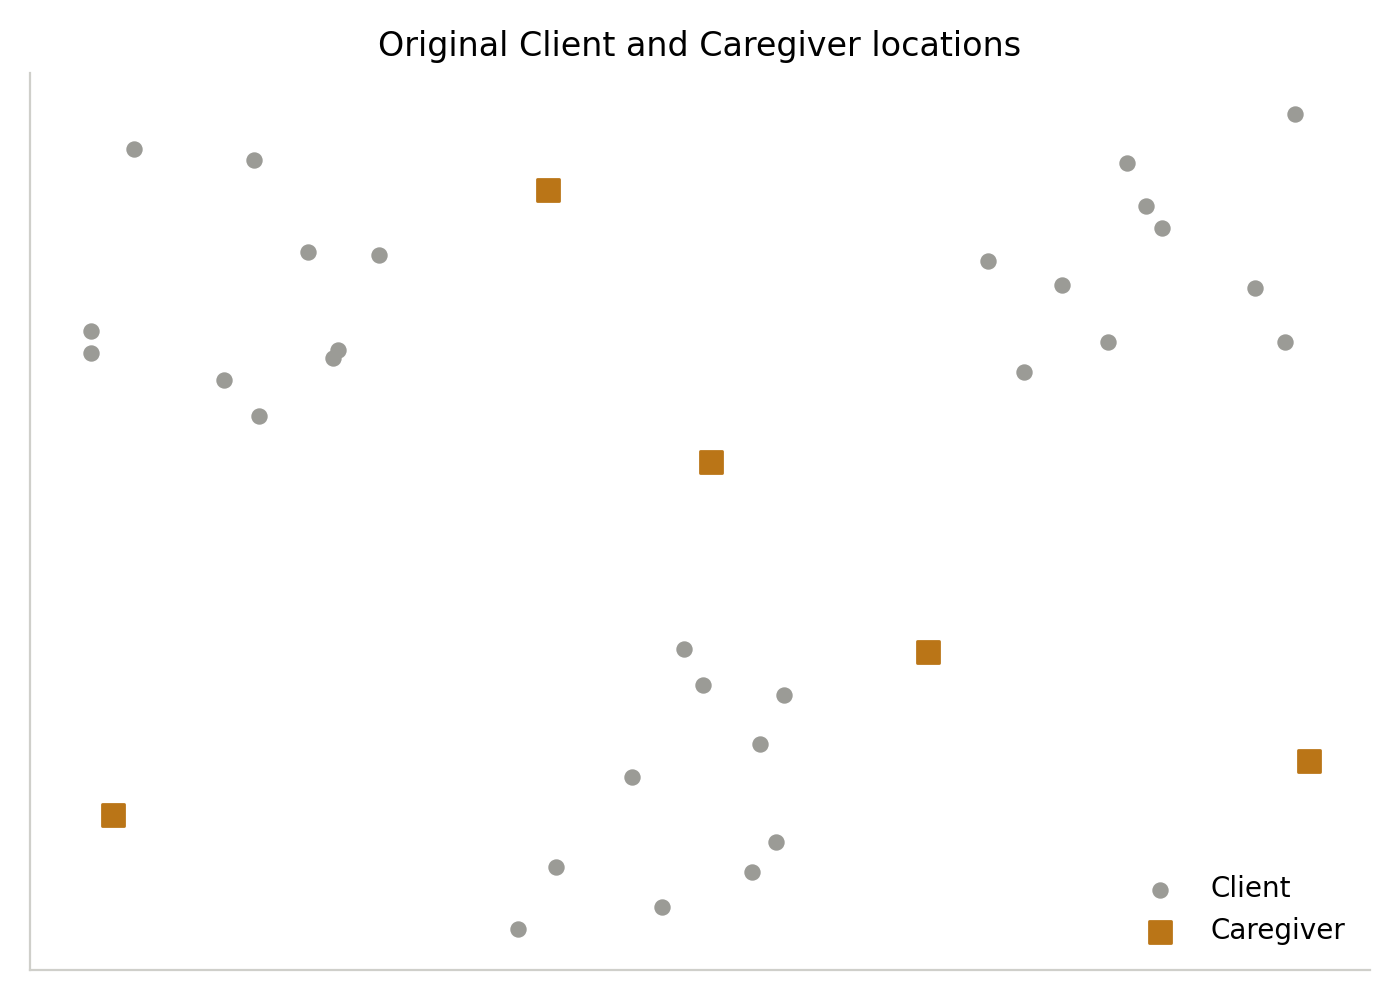
\includegraphics[width=0.65\textwidth]{01_raw_scatter.png}
	\caption{Example Initial State}
	\label{fig:init}
\end{figure}

At this point in the process, certain information is known about each point in this scatter plot. The shift pattern, working days, and driving ability of each caregiver is known at this point, and the distance between each caregiver and each client is also known. Unfortunately, the distance between caregivers is at this point unknown, and will have to be imputed at some point in the pipeline. Similarly, the demands of and the list of caregivers known to each client is known, as well as the distance from any client to any other client. The first step taken is to totally enumerate all feasible caregiving units based on caregiver shift patterns. In the example in Figure \ref{fig:shifts}, a coupling is made between c3 and c4, as c3's shift ends before c4's starts. This means c3 and c4 can be treated together as one, full-time equivalent caregiver. Feasible units are then made with all caregivers regardless of shift pattern individually as solo units, all couples individually as solo units, and any pairing between caregivers and/or couples where one shift fully contains the other and at least one equivalent full-time member of the potential pairing is listed as a driver. Assuming all caregivers are drivers in the example in Figure \ref{fig:shifts}, the only infeasible pair is (c3, c4), with all other combinations of two caregivers feasible and the couple (c3, c4) a feasible member of a pair with all remaining caregivers. 

\begin{figure}[H]
	\centering
	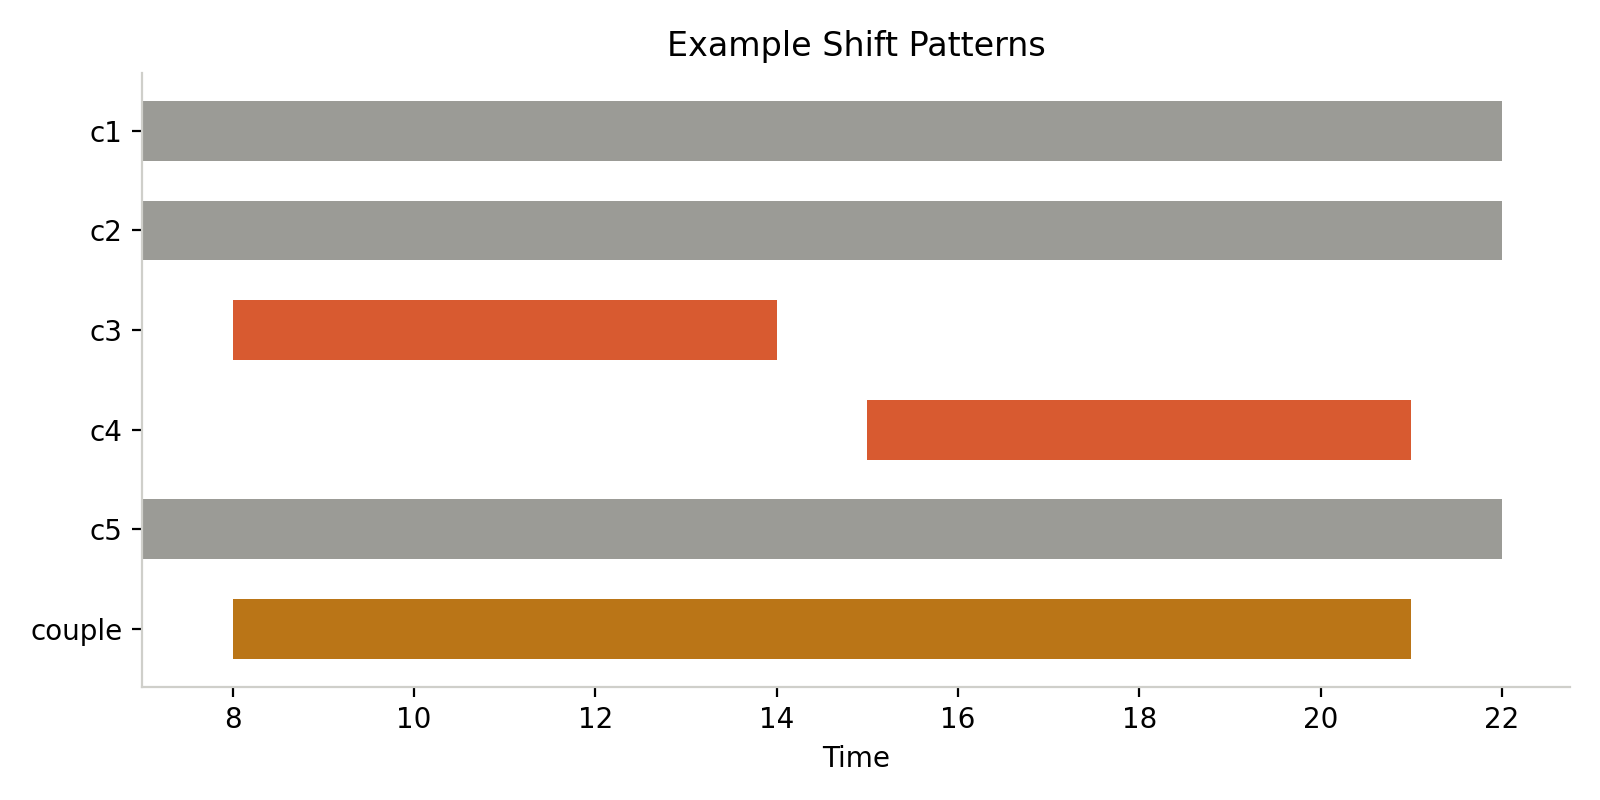
\includegraphics[width=0.5\textwidth]{02_unit_building.png}
	\caption{Example Caregiver Shift Patterns}
	\label{fig:shifts}
\end{figure}

From this point, it is necessary to identify clusters of clients to determine the localities which will be used for the model. This further enables the ability to model where demands are concentrated, as well as assign a home locality for each caregiver according to their respective nearest clients. To do this, bottom-up hierarchical clustering is employed, as actual client locations are unknown at this point, but travel times between clients are known. Bottom-up hierarchical clustering involves starting with each client in its own cluster, then iteratively merging the two nearest clusters until only one cluster remains. To ensure robustness, inter-cluster distance in this case was determined by the farthest distance between a member of each respective cluster. This process can be visualized by a dendrogram, a tree that shows the merging of clusters at each iteration. Since this clustering process is iterative, any desired number of clusters can be taken by pruning the dendrogram at the appropriate point; in the example from Figure \ref{fig:clust} that is the point at which there are three clusters remaining, while in the implemented version of the model the chosen number is eight.

\begin{figure}[H]
	\centering
	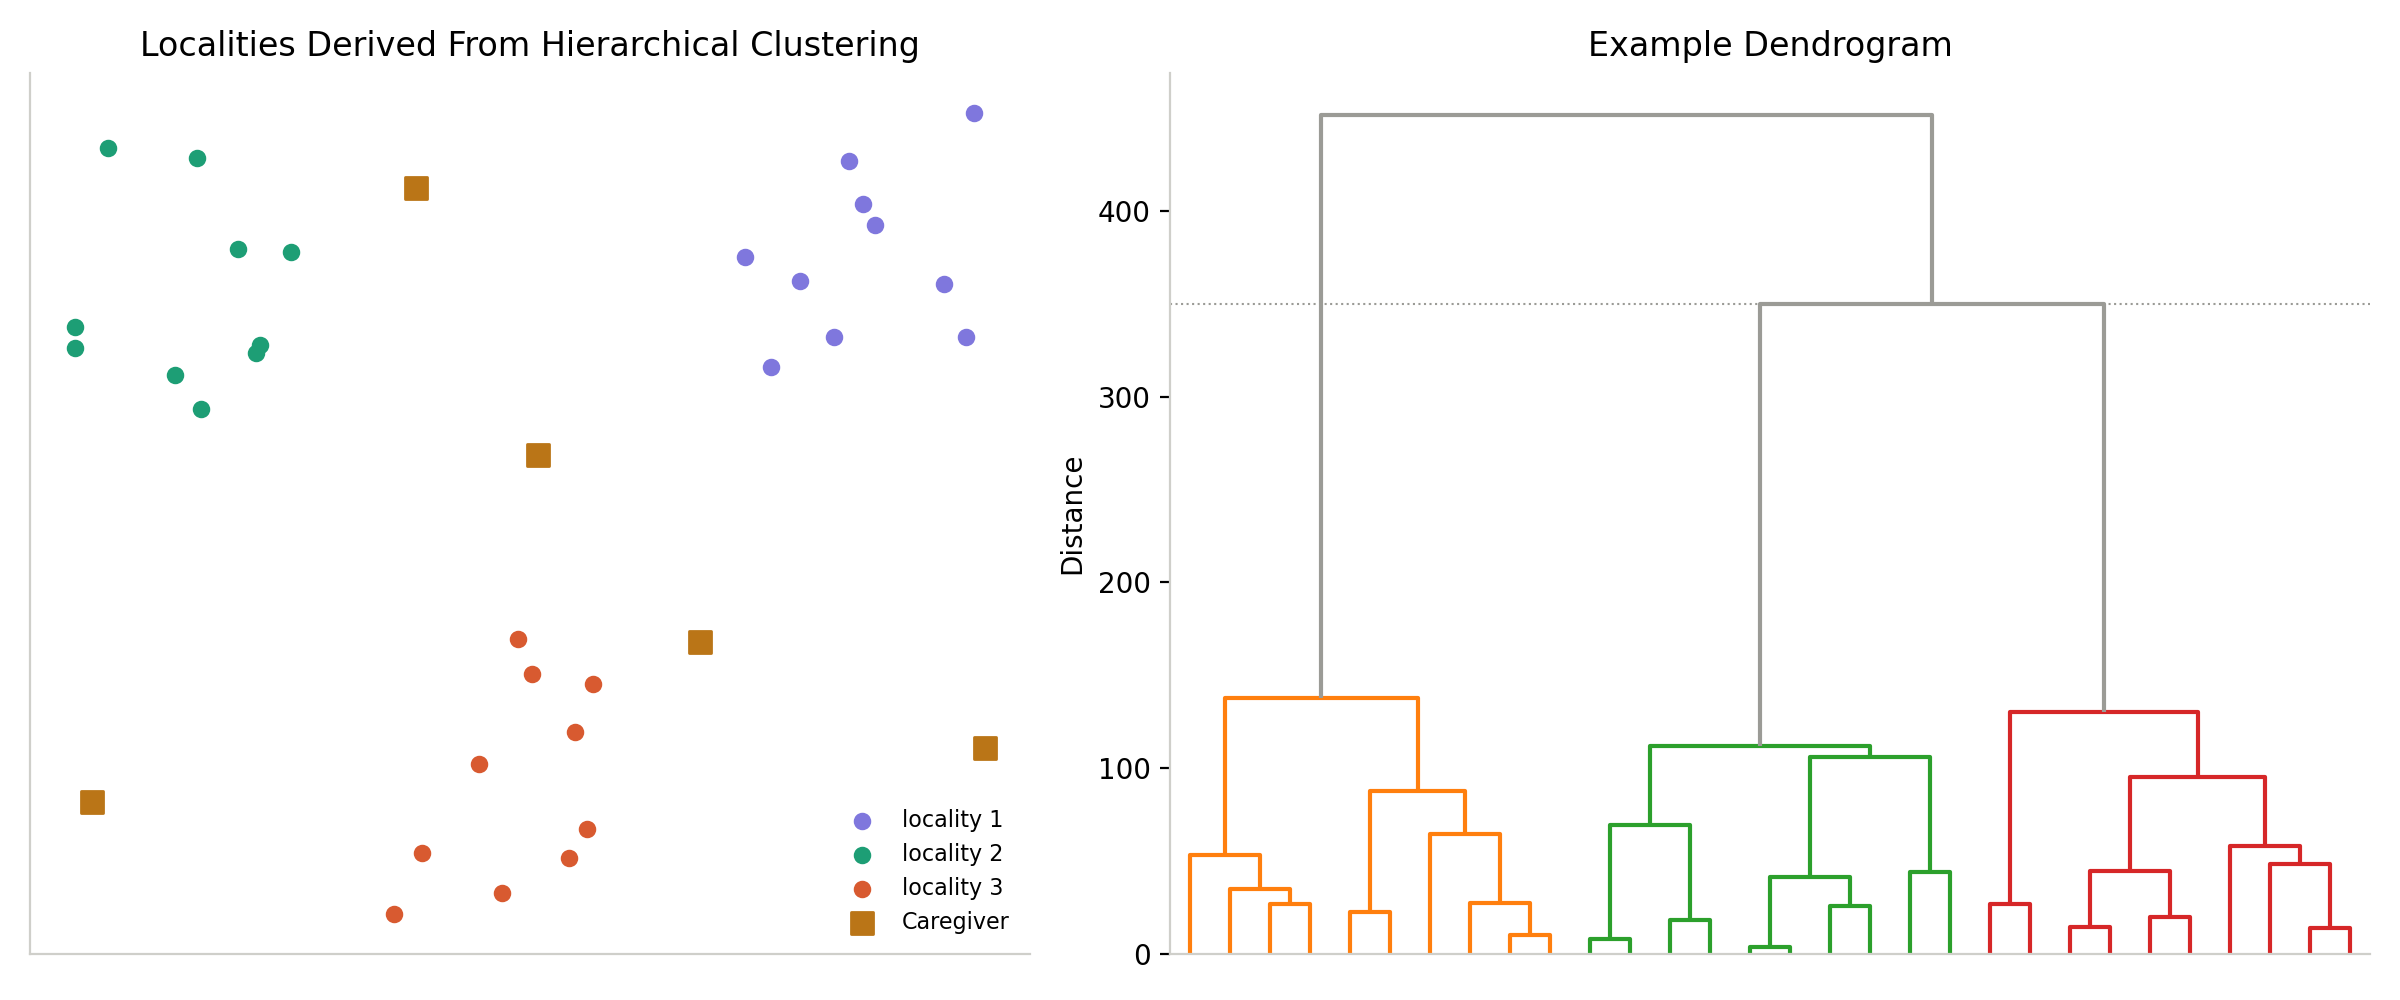
\includegraphics[width=0.65\textwidth]{03_clustering_and_dendrogram.png}
	\caption{Example Client Clusters}
	\label{fig:clust}
\end{figure}

With localities assigned, it is now necessary to calculate the missing caregiver travel parameters. In a further effort to ensure robustness, the distance from a caregiver to a locality is taken as the furthest observed distance from that caregiver to a client assigned to the given locality. The distance between two caregivers is calculated from the known values of the distance between each caregiver and their respective nearest client plus the known value of the distance between those two clients. This also ensures distance symmetry, i.e. the distance from caregiver one to caregiver two will be the same as the distance from caregiver two to caregiver one. The distance required to form a unit is then taken as the unique sum of distances between each caregiver in a unit. For a single member unit this will be zero, for a two member unit this will be the single computed distance between the two members, and for a three member unit this will be the three computed distances between each unique pair of unit members. This process is illustrated in Figure \ref{fig:dist}.

\begin{figure}[H]
	\centering
	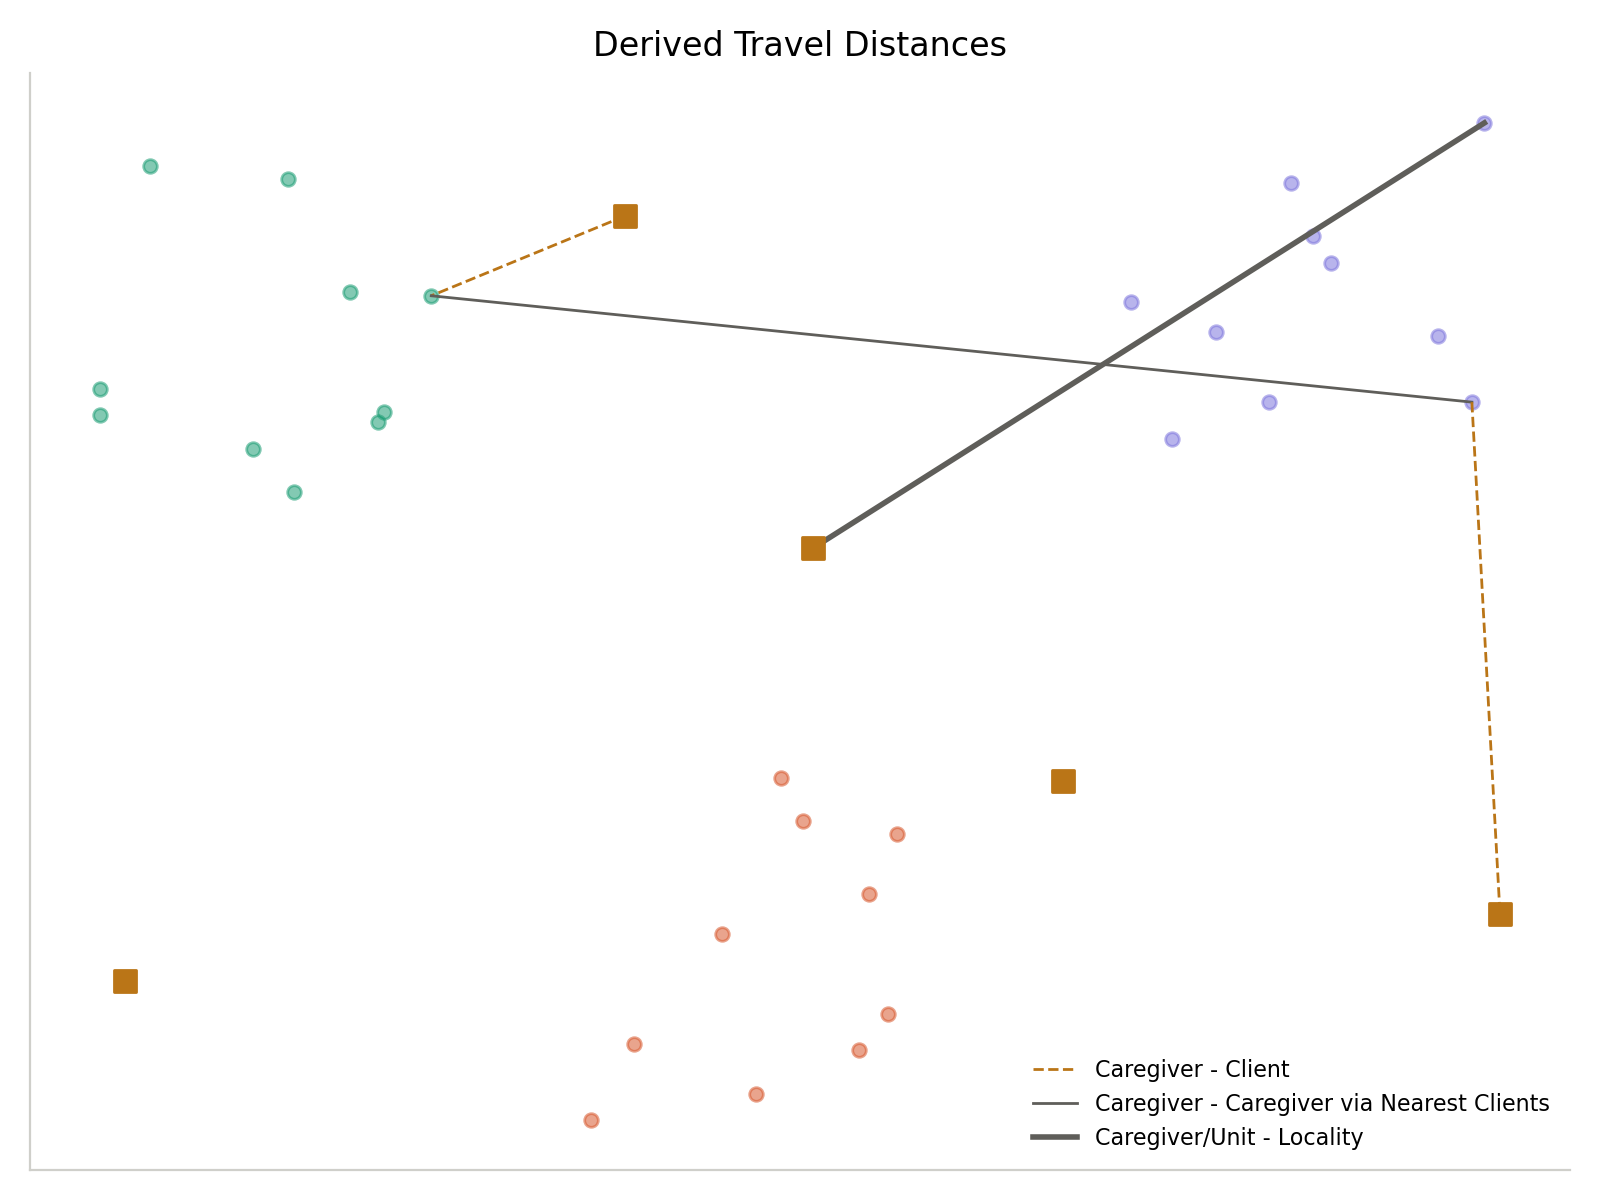
\includegraphics[width=0.65\textwidth]{04_travel_distances.png}
	\caption{Example Travel Time Construction}
	\label{fig:dist}
\end{figure}

With this, all required parameters are known, and the model as described earlier can be built and run. As mentioned, the model will produce up to five unique candidate solutions for the unit assignments of caregivers on a day-to-day basis as a preliminary to a routing and scheduling heuristic. While the model will provide both unit assignments and locality assignments for each chosen unit, locality assignments are ignored by the downstream process. The locality assignment is still necessary for the model, as it ensures that the geospatial ramifications of a candidate caregiver assignment are properly considered, especially as an objective of the model is to minimize unpaid caregiver travel time. A candidate solution will then have $x_u^d = 1$ if unit $u$ is assigned on day $d$, with $z_{ul}^d = 1$ if if unit $u$ is assigned to locality $l$ on day $d$. An example of this is found in Figure \ref{fig:sol}.

\begin{figure}[H]
	\centering
	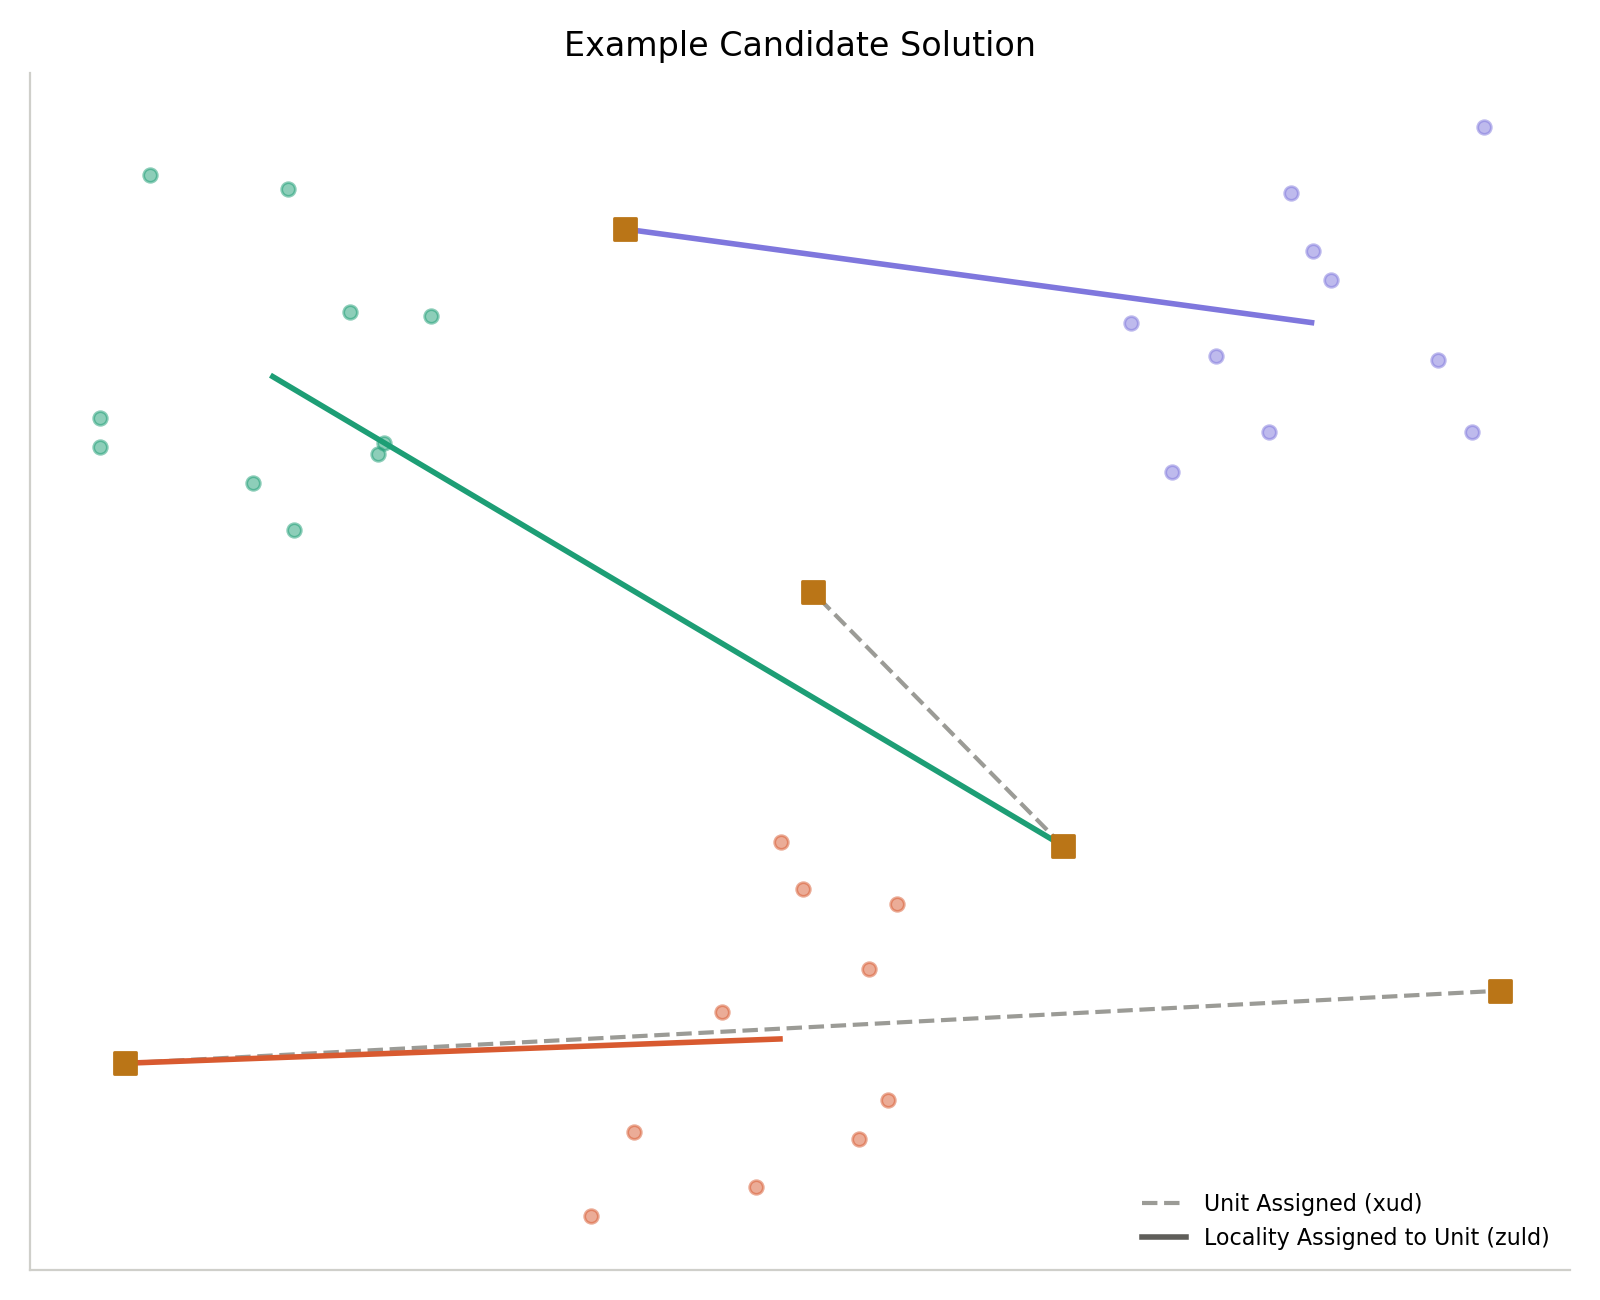
\includegraphics[width=0.65\textwidth]{05_assignment.png}
	\caption{Example Candidate Assignment}
	\label{fig:sol}
\end{figure}

\clearpage

\section{Results}
\label{sec:res}
The Home Healthcare provider in question provided data for two weeks of visits to be routed and scheduled, available caregivers and their relevant traits, anonymized client information, and a travel matrix containing travel times for client-client and caregiver-client travel. A preprocessing script written in Python is used to derive all relevant model parameters and write them to a pickle file. The model is then implemented in a separate script written in Python and using Gurobi Optimizer using its Python API. The model is optimized according to the multi-objective framework described in Chapter \ref{sec:meth}. The script then checks each of the five generated solutions to ensure that no duplicate solutions were returned; in the test case, four unique solutions were generated. Unique solutions are then written to separate csv files in a standard format. 

Implementation was done on an Apple M2-chipped machine running MacOS with 8 GB of RAM. The preprocessing script handled the preprocessing of the two week dataset and ran in approximately 5 seconds, while the modelling script created candidate caregiver assignments for the same two week horizon and ran in approximately 12 seconds. Four unique candidate assignments were generated according to the data provided. These candidates were then tested with the existing Routing and Scheduling heuristic.
\subsection{Effect on Downstream Routing and Scheduling Process}
Candidate solutions were used to generate corresponding routes for the first day in the data. The first three each left eight of the day's 310 visits unallocated (2.58\% unallocated), with two instances of these involving seven of the day's 125 two caregiver-requiring visits (5.6\%) and one of the day's 185 single caregiver-requiring visits (2.92E-3\%) and a third involving all eight unallocated visits belonging to the two caregiver-requiring category (6.4\%). The final candidate solution involved only six unallocated visits of the 310 total (1.94\%), all of which fell in the two caregiver-requiring category (4.8\%). 

Another performance indicator to consider is the allocation of caregiver shift time to visits versus driving and idle time. Each candidate assignment yielded routes that devoted approximately 61\% of caregiver shift time to visits, with approximately 12\% of the remaining time spent in transit to visits and approximately 27\% classified as time spent idle. These values ranged from 59.9\% to 61.32\%, 11.55\% to 12.54\%, and 26.37\% to 28.54\% across generated routings respectively. A table with relevant summarized results from the routing and scheduling process is given in Table \ref{tab:restab}, with all times given in hours and minutes.

\begin{table}[H]
	\begin{center}
		\caption{Relevant Assignment-Derived Routing and Scheduling Results (310 Total Visits, 125 Require Pair Units, 185 Require Solo Units)}
		\label{tab:restab}
		\setlength{\tabcolsep}{3.75pt}
		\begin{tabular}{cccccccc}
			\makecell{Candi-\\date\\Solution} & \makecell{Unallo-\\cated\\Visits} & \makecell{Unallo-\\cated\\Single-\\Caregiver\\Visits} & \makecell{Unallo-\\cated\\Double-\\Caregiver\\Visits} & \makecell{Total (\%)\\Care-\\giving\\Time} & \makecell{Total (\%)\\Travel\\Time} & \makecell{Total (\%)\\Idle Time} & \makecell{Total\\Routing\\Time}\\
			\toprule
			\textbf{1} & 8 & 1 & 7 & 182:45 (61.32\%) & 36:43 (12.32\%) & 78:35 (26.37\%) & 298:03 \\
			\textbf{2} & 8 & 0 & 8 & 183:00 (61.06\%) & 35:19 (11.78\%) & 81:23 (27.25\%) & 299:42 \\
			\textbf{3} & 8 & 1 & 7 & 182:45 (59.90\%) & 35:15 (11.55\%) & 87:04 (28.54\%) & 305:04 \\
			\textbf{4} & 6 & 0 & 6 & 184:30 (60.72\%) & 38:06 (12.54\%) & 81:14 (26.74\%) & 303:50 \\
		\end{tabular}
	\end{center}
\end{table}

These effects were not, however, evenly distributed among caregivers, as several routes saw no time classified as idle while others saw values as high as eight hours 51 minutes. Visit time similarly saw wide ranges within routings, with a maximum observed difference of 10 hours and 45 minutes between the maximum observed 12 hours of visit time on a route compared to the equivalent minimum of one hour 15 minutes observed. Transit times were typically better distributed between routes, with most routes involving somewhere between two and a half hours and 30 minutes of transit time. Of note is that with regard to these inter-route comparisons is that they are influenced by routes represented entirely by part-time caregivers, which exacerbates the differences. Furthermore, the candidate assignments put forward by this work are made in an effort to minimize expected transit time with considerations for the geospatial distribution of demand, but do not consider these disparities and do not assign caregiving units localities or visits that carry over to the downstream routing and scheduling heuristic. Full results from the terminal output of the downstream routing and scheduling heuristic as applied to the caregiver assignments derived by the model can be found in \ref{app:two}.
\clearpage

\section{Conclusion}
\label{sec:conc}
Home Healthcare as a domain presents a complex operational system of growing social relevance. Operations Research literature has recognized this and devoted a significant amount of research effort to exploring, among other aspects, how the domain's routing and scheduling of caregivers to visits can be optimized under the framework of the Home Healthcare Routing and Scheduling Problem. This work is framed as a component piece to a further application and potential extension to this existing literature in conjunction with a potentially forthcoming publication from this work's supervisor. 

This work puts forth a multi-objective Mixed-Integer Linear Programming formulation for a preliminary caregiver unit assignment, meant to reduce the complexity necessary of a downstream Routing and Scheduling heuristic. This formulation is built around the factors most relevant to the particular application scenario in which it is developed, namely the roughly equivalent share of visits requiring caregiver pairs and solo caregivers; the unequal geospatial distribution of its caregivers, clients, and visits requiring caregiver pairs and solo caregivers; and the non-homogeneity of caregiver driving ability and shift patterns. Due to the relative homogeneity of other caregiver traits and abilities, the specifics of client preference for caregivers, factors relevant to a similar work in a different application context such as caregiver skill sets, caregiver gender and client preference thereof, and further client preferences are not considered in this work. The model described herein takes a multi-objective approach, namely optimizing for the maximization of potential familiar visits and minimization of potential caregiver travel. As the actual observed values of these objectives are beyond the scope of this work and instead a question of the downstream Routing and Scheduling heuristic, the model put forth herein attempts to optimize for their respective ceilings. 

There exist certain limitations to the model developed in this report. As a preliminary step, the model described herein does little on its own to further the understanding of the Home Healthcare Routing and Scheduling Problem, though as a system it does take its place in the literature as one of several multi-step processes combining exact and heuristic methods to more efficiently find solutions. A limitation related both to this context as a preliminary step and the results of this work is that it alone does not directly optimize for the objectives of Home Healthcare providers. This is mitigated in its optimization for downstream potential realization of objectives, but without subsequent routing and scheduling steps, the work achieves little of novelty with respect to existing Operations Research literature. Furthermore, as mentioned previously, this work is very much tailored to the specific application environment in which it is developed, so factors that might influence an optimized caregiver pairing assignment in other contexts such as caregiver qualifications, gender, or suitability to client preferences other than familiarity are not considered. Additionally, the objectives for which it optimizes are chosen in consultation with representatives of the provider, whose priorities may differ from those of other providers. Indeed, literature evidence would suggest a wide range of potential objectives in a general Home Healthcare context not considered herein. Finally, a limitation of this work beyond that of its scope and specificity is the limited amount of testing conducted in relation to its efficacy. Testing was limited to a single, two week instance of data with regard to building caregiver unit assignments, while assignments' effects on downstream routing and scheduling saw further limited testing to the instance of a single day. Analysis of this downstream effect is limited by a lack of data on the performance of the tool developed in relation to this work and a lack of corresponding data for whatever incumbent process this tool is developed to replace. This greatly limits the ability to meaningfully evaluate the model's efficacy with any reasonable degree of confidence.

Some further work related both directly to this model and to other future preliminary caregiver assignment steps are proposed. With regard to this work in particular, caregiver assignments may be further improved by more strictly defining feasible caregiver units. Namely, the current rule for determining feasible pairs is to determine whether one caregiver's or equivalent caregiver coupling's working hours contain the potential partner caregiver's or caregiver coupling's. This can be more strictly defined as ensuring that each relevant shift or equivalent shift starts and ends within a certain time window relative to each other. This would limit considered pair assignments to only those which would occupy all involved caregivers' entire shifts, reducing the need for synchronization and/or ad-hoc planning when one half of an assigned pair is no longer working. Observationally, the downstream routing process left several two-caregiver visits unallocated in a limited test sample, which may have been due to the scheduled absence of an otherwise paired caregiver unaccounted for in the assignment model. Another potential adjustment to the model meant to address a potential shortcoming in pair assignments, and especially pair assignments involving a coupling of part-time caregivers, would be to increase the tolerated deviation in the constraints related to share of assignments allocated to pair (and consequently solo) units, including those related to geospatial distribution. Specifically, there is potential that increasing the upper bound on the number of daily pair assignments selected may allow for the increased assignment of pair units, which may in turn improve downstream results. That said, this adjustment, especially as it relates to the geospatial constraints, may instead make solutions less valuable by requiring further travel and inadequately covering certain demand(s).

Further work may also consider additional factors beyond those considered in this model. Factors such as potential caregiver workload and overtime could be taken into account by future work in an effort to ensure caregiver satisfaction. One approach to do this on a locality basis would be to consider the number of a given type of visit minutes in a locality per the number of appropriate units assigned to that locality, which could be linearized by taking the inverse measure (number of appropriate units per corresponding visit minutes) and swapping maximization and minimization in the objective case or greater than and lesser than in the constraint case. A similar consideration could be taken to ensure parity in caregiver workload, though this might require more specific consideration of caregiver shift patterns. A note on these considerations is that, as with the objectives of this model, the assignment of caregiver units does not prescribe their realized value, and corresponding modelling efforts must therefore reflect these measures' potential in downstream processes.

This work concerns the development of a tool which assigns caregivers in a certain Home Healthcare provider to units composed of either one or two concurrent active members as a preliminary step for day-to-day caregiver routing and scheduling made with consideration for the specific Home Healthcare context for which it is developed and the broader context of the literature. As a standalone work, it is a rather textbook example of an application of the General Assignment Problem, with little to differentiate it from other such applications in formulation or in methodology. However, this work does represent a component piece to a broader application and potential expansion of the Operations Research literature relating to the Home Healthcare Routing and Scheduling Problem.

\clearpage

%the entries have to be in the file literature.bib
\bibliography{literature}
\clearpage

\section*{AI Disclosure}
\textbf{Proofing:} Generative AI was used to assist in spelling, grammar, and other checking in the following ways
\begin{itemize}
	\item [ChatGPT and Claude] [13 July - 10 August] [Debugging of Python code]
	\item [ChatGPT and Claude] [5 - 10 August] [Debugging of LaTeX code]
	\item [Claude] [10 August] [Addition of Python Code Comments]
\end{itemize}

\appendix
\section*{Appendices}
\addcontentsline{toc}{section}{Appendices}

\section{Link to Additional Materials}
\label{app:one}

All code discussed in this report has been published via the GitHub repository linked below:

\href{https://github.com/mpannenkoeken/msc-hhrsp}{https://github.com/mpannenkoeken/msc-hhrsp}

\section{Full Test Routing Results}
\label{app:two}

\begin{verbatim}
	===================================================

 

Pairing 1

 

Day   | Route |   Care | Drive | Idle

-------+-------+--------+-------+-------

[Mon,1]|     1 |   8:15 |  1:39 |  1:31

[Mon,1]|     1 |  11:30 |  1:39 |  1:31

[Mon,1]|     2 |   8:00 |  1:21 |  3:24

[Mon,1]|     3 |   6:00 |  1:36 |  5:39

[Mon,1]|     3 |   8:00 |  1:36 |  5:39

[Mon,1]|     4 |   7:30 |  2:14 |  1:56

[Mon,1]|     4 |  10:30 |  2:14 |  1:56

[Mon,1]|     5 |   7:30 |  3:10 |  1:02

[Mon,1]|     5 |  11:15 |  3:10 |  1:02

[Mon,1]|     6 |   7:00 |  1:00 |  6:13

[Mon,1]|     6 |   8:15 |  1:00 |  6:13

[Mon,1]|     7 |   6:30 |  2:13 |  3:40

[Mon,1]|     7 |   9:15 |  2:13 |  3:40

[Mon,1]|     8 |   5:30 |  0:43 |  4:17

[Mon,1]|     9 |   6:00 |  1:47 |  2:49

[Mon,1]|     9 |   7:30 |  1:47 |  2:49

[Mon,1]|    10 |   2:30 |  0:31 |  0:00

[Mon,1]|    11 |   8:15 |  0:58 |  5:22

[Mon,1]|    12 |   3:15 |  0:34 |  0:00

[Mon,1]|    13 |   6:45 |  1:06 |  7:00

[Mon,1]|    14 |  11:30 |  1:13 |  1:04

[Mon,1]|    15 |   1:45 |  0:32 |  1:15

[Mon,1]|    16 |   6:45 |  0:44 |  1:19

[Mon,1]|    17 |   4:30 |  0:39 |  8:51

[Mon,1]|    18 |   5:00 |  0:29 |  5:16

[Mon,1]|    19 |   4:00 |  0:35 |  0:23

-------+-------+--------+-------+-------

                        | 182:45 | 36:43

 

Unallocated visits

2-carer: 7

1-carer: 1

 

======================================================

 

Pairing 2

 

Day   | Route |   Care | Drive | Idle

-------+-------+--------+-------+-------

[Mon,1]|     1 |   5:30 |  1:13 |  0:35

[Mon,1]|     1 |   5:30 |  1:13 |  0:35

[Mon,1]|     2 |   5:30 |  0:43 |  4:17

[Mon,1]|     3 |   7:30 |  2:28 |  4:00

[Mon,1]|     3 |   9:00 |  2:28 |  4:00

[Mon,1]|     4 |   8:15 |  1:33 |  1:20

[Mon,1]|     4 |  10:30 |  1:33 |  1:20

[Mon,1]|     5 |   7:45 |  1:15 |  3:45

[Mon,1]|     6 |   5:00 |  1:00 |  0:00

[Mon,1]|     6 |   5:15 |  1:00 |  0:00

[Mon,1]|     7 |   7:15 |  0:54 |  6:00

[Mon,1]|     7 |   7:15 |  0:54 |  6:00

[Mon,1]|     8 |   7:45 |  2:35 |  1:37

[Mon,1]|     8 |  10:45 |  2:35 |  1:37

[Mon,1]|     9 |   7:15 |  2:30 |  2:39

[Mon,1]|     9 |  10:15 |  2:30 |  2:39

[Mon,1]|    10 |   4:30 |  0:57 |  8:43

[Mon,1]|    11 |   6:30 |  1:03 |  6:15

[Mon,1]|    12 |   2:30 |  0:31 |  0:00

[Mon,1]|    13 |   8:15 |  0:58 |  5:22

[Mon,1]|    14 |   4:15 |  0:56 |  0:00

[Mon,1]|    15 |   6:45 |  1:09 |  6:57

[Mon,1]|    16 |  11:30 |  1:13 |  1:04

[Mon,1]|    17 |   6:45 |  0:44 |  1:19

[Mon,1]|    18 |   5:30 |  0:47 |  8:35

[Mon,1]|    19 |   6:15 |  0:37 |  4:44

-------+-------+--------+-------+-------

                        | 183:00 | 35:19

 

Unallocated visits

2-carer: 8

1-carer: 0

 

======================================================

 

Pairing 3

 

Day   | Route |   Care | Drive | Idle

-------+-------+--------+-------+-------

[Mon,1]|     1 |   7:45 |  1:03 |  5:14

[Mon,1]|     2 |   6:00 |  1:23 |  6:02

[Mon,1]|     2 |   7:30 |  1:23 |  6:02

[Mon,1]|     3 |   9:00 |  1:54 |  1:19

[Mon,1]|     3 |  12:00 |  1:54 |  1:19

[Mon,1]|     4 |   7:45 |  2:44 |  1:13

[Mon,1]|     4 |  11:00 |  2:44 |  1:13

[Mon,1]|     5 |   7:30 |  0:54 |  6:25

[Mon,1]|     5 |   8:00 |  0:54 |  6:25

[Mon,1]|     6 |   5:45 |  1:17 |  5:43

[Mon,1]|     7 |   6:30 |  1:45 |  4:02

[Mon,1]|     7 |   8:30 |  1:45 |  4:02

[Mon,1]|     8 |   6:30 |  1:36 |  3:00

[Mon,1]|     8 |   7:45 |  1:36 |  3:00

[Mon,1]|     9 |   6:45 |  1:17 |  6:02

[Mon,1]|    10 |   5:30 |  2:23 |  2:01

[Mon,1]|    10 |  10:15 |  2:23 |  2:01

[Mon,1]|    11 |   1:30 |  0:15 |  0:00

[Mon,1]|    12 |   8:15 |  0:58 |  5:22

[Mon,1]|    13 |   3:45 |  0:26 |  0:00

[Mon,1]|    14 |  11:30 |  1:15 |  0:57

[Mon,1]|    15 |   1:15 |  0:20 |  1:40

[Mon,1]|    16 |   6:45 |  0:44 |  1:19

[Mon,1]|    17 |   6:15 |  1:09 |  6:23

[Mon,1]|    18 |   7:00 |  0:57 |  4:21

[Mon,1]|    19 |   2:30 |  0:16 |  1:59

-------+-------+--------+-------+-------

                        | 182:45 | 35:15

 

Unallocated visits

2-carer: 7

1-carer: 1

 

======================================================

 

Pairing 4

 

Day   | Route |   Care | Drive | Idle

-------+-------+--------+-------+-------

[Mon,1]|     1 |   6:45 |  2:02 |  4:45

[Mon,1]|     1 |   7:45 |  2:02 |  4:45

[Mon,1]|     2 |   8:15 |  1:32 |  1:23

[Mon,1]|     2 |  11:15 |  1:32 |  1:23

[Mon,1]|     3 |   7:45 |  1:03 |  5:14

[Mon,1]|     4 |   6:00 |  1:20 |  3:40

[Mon,1]|     4 |   6:15 |  1:20 |  3:40

[Mon,1]|     5 |   6:15 |  2:09 |  2:49

[Mon,1]|     5 |  10:30 |  2:09 |  2:49

[Mon,1]|     6 |   4:00 |  0:37 |  8:08

[Mon,1]|     7 |   6:45 |  2:31 |  1:33

[Mon,1]|     7 |  10:30 |  2:31 |  1:33

[Mon,1]|     8 |   7:45 |  2:21 |  2:26

[Mon,1]|     8 |  10:30 |  2:21 |  2:26

[Mon,1]|     9 |   7:30 |  1:47 |  4:46

[Mon,1]|     9 |   8:45 |  1:47 |  4:46

[Mon,1]|    10 |   1:30 |  0:15 |  0:00

[Mon,1]|    11 |   9:00 |  1:26 |  4:09

[Mon,1]|    12 |   3:30 |  0:46 |  0:00

[Mon,1]|    13 |   5:30 |  1:09 |  5:02

[Mon,1]|    14 |  11:30 |  1:15 |  0:57

[Mon,1]|    15 |   1:30 |  0:33 |  1:12

[Mon,1]|    16 |   6:45 |  0:44 |  1:19

[Mon,1]|    17 |   7:00 |  1:02 |  6:02

[Mon,1]|    18 |   8:45 |  1:30 |  5:04

[Mon,1]|    19 |   3:00 |  0:22 |  1:23

-------+-------+--------+-------+-------

                        | 184:30 | 38:06

 

Unallocated visits

2-carer: 6

1-carer: 0
\end{verbatim}
\end{document}
